\documentclass[12pt]{article}
%\usepackage[spanish]{babel}
\usepackage[utf8]{inputenc}
\usepackage{amsmath}
\usepackage{amsfonts}
\usepackage{amssymb}
\usepackage{graphicx}
\usepackage{hyperref}
\usepackage{doi}
\usepackage{mathtools}
\usepackage{float}
\usepackage[colorinlistoftodos]{todonotes}
\usepackage[letterpaper, margin=1.in]{geometry}
%\usepackage[version=3]{mhchem}

\begin{document}

\begin{titlepage}

\newcommand{\HRule}{\rule{\linewidth}{0.5mm}}

\center

\textsc{\LARGE Universidad de los Andes}\\[1.5cm]
\textsc{\Large Departamento de F\'isica}\\[0.5cm]
\textsc{\large Biolog\'ia Sint\'etica}\\[0.5cm] 

\HRule \\[0.4cm]
{ \huge \bfseries Proyecto}\\[0.4cm]
\HRule \\[1.5cm]
 

\Large \emph{Autores:}\\
Manuela \textsc{Vanegas Ferro}\\
Juan David \textsc{Estupi\~n\'an M\'endez}\\
Luis Alberto \textsc{Guti\'errez L\'opez}\\[2cm]

\Large \emph{Profesor:}\\
Juan Manuel \textsc{Pedraza Leal}\\[3cm]


{\large Mayo 21 de 2015}\\[2cm]

\vfill

\end{titlepage}

\tableofcontents
\pagebreak

\begin{abstract}
  Your abstract\cite{kressler01} \cite{cleland67} \cite{turlings95} \cite{sallaud09} \cite {kirby09} \cite{harada09a} \cite{harada09b} \cite{crocker80} \cite{engerberg-kulka04} \cite {alon06}.
\end{abstract}

\section{Introducci\'on}
El uso de sistemas naturales en el campo de la biolog\'ia sint\'etica ha sido la principal forma de generar nuevos circuitos y comportamientos. Por ejemplo, hay sistemas que usan ciertas plantas para protegerse del ataque de herv\'ivoros, produciendo qu\'imicos vol\'atiles que atraen a los enemigos naturales de los herb\'ivoros. Este es el caso de \emph{Nicotiana attenuata}, o tabaco coyote. Esta planta, cuando siente da\~no por hervibor\'ia, libera bergamoteno para atraer a insectos del g\'enero \emph{Geocoris}, los cuales son depredadores de aproximadamente 65 especies distintas.\\
Debido a que este sistema es muy espec\'ifico, este proyecto busca hacerlo m\'as general, peritiendo que muchas especies de plantas se puedan proteger de una forma m\'as eficiente de los herv\'iboros, sin necesidad de usar qu\'imicos insecticidas. De esta forma, buscamos modificar a la bacteria \emph{Escherichia coli} para que produzca Bergamoteno cuando ella detecte da\~no por herbivor\'ia. Este proyecto presenta el desafio de controlar la producci\'on de Farnesil pirofosfato (FPP) porque es t\'oxico para \emph{E. coli}, adem\'as se busca optimizar la producci\'on de bergamoteno de tal forma que no sea da\~nino para la planta a largo plazo.

\section{Modelo Matem\'atico}
\label{sec:model}
\subsection{dise\~no}
\begin{figure}[H]
  \centering
  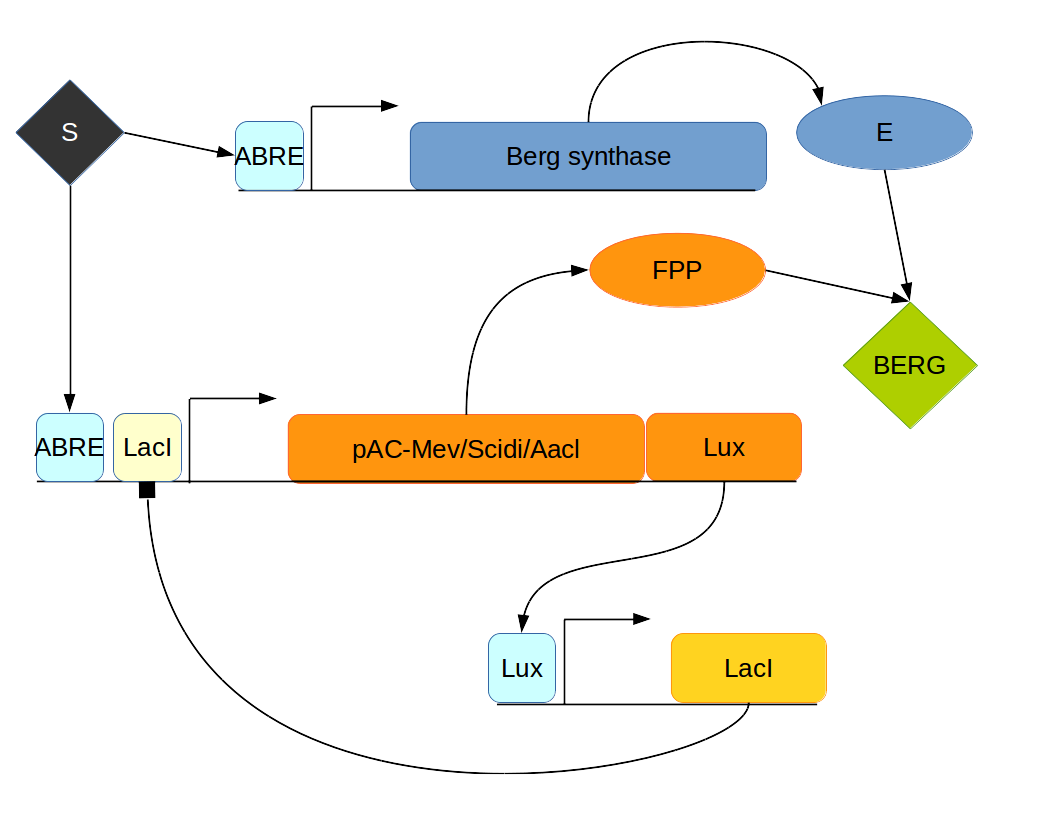
\includegraphics[width=0.6\textwidth]{Circuit.png}
  \caption{\label{fig:Circuit} Interconecciones entre los genes que se van a usar en el modelo}
\end{figure}
El siguiente modelo cuenta con 2 partes. La primera se refiere a la produce la enzima \emph{Bergamoteno sintetasa} (E en la figura \ref{fig:Circuit}). La otra parte requiere del pl\'asmido \emph{pAC-Mev/Scidi/Aacl}, que sintetiza las enzimas necesarias para llevar \emph{Acetil CoA} a FPP (Z en la figura \ref{fig:Circuit}). Ambas partes tienen un promotor activado por la se\~nal de da\~no. Este es el promotor \emph{ABRA} que se encuentra en organismos vegetales y est\'a asociado a la recepci\'on y señalizaci\'on de \'acido absc\'icico (ABA). Adem\'as, el circuito del pl\'asmido presenta un promotor de inhibici\'on de LacI, el cual es producido por este mismo circuito para generar un feedback negativo. De esta manera, se busca que la producci\'on de la enzima Z sea de manera oscilatoria, y as\'i limitar la concentraci\'on de FPP.

\subsection{Ecuaciones de Hill}

Se model\'o la parte transcripcional como se ha hecho en clase y est\'a explicado en \cite{alon06}. Consideramos que el ADN total del gen a transcribir $\text{D}_{\text{T}}$ es constante, es decir:

\begin{equation} \label{eq:D_T}
[\text{D}_{\text{T}}]=[\text{D}]+[\text{DS}]+[\text{DI}]+[\text{DIS}],
\end{equation}

Donde $[\text{D}]$ representa el ADN libre, $[\text{DIS}]$ el ADN unido tanto al represor I como al activador S, $[\text{DS}]$ el unido al activador, y $[\text{DI}]$ el unido al represor.

Para realizar balance detallado se consideraron las siguientes ecuaciones qu\'imicas, las cuales son equivalentes al diagrama del inicio  de la primera tarea del curso.

%\begin{align}
%\ce{[D] + [S]} &\ce{<=>[\ce{k_{S+}}][\ce{k_{S-}}] [DS]}, \label{eq:rchem1}\\ 
%\ce{[D] + [I]} &\ce{<=>[\ce{k_{I+}}][\ce{k_{I-}}] [DI]}, \label{eq:rchem2}\\
%\ce{[DS] + [I]} &\ce{ <=>[\ce{k_{I+}}][\ce{k_{I-}}] [DIS]}, \label{eq:rchem3}\\ 
%\ce{[DI] + [S]} &\ce{<=>[\ce{k_{S+}}][\ce{k_{S-}}] [DIS]}. \label{eq:rchem4}
%\end{align}

Donde las $k$ son las constantes de las respectivas reacciones y se define la constante de disociaci\'on como $K = \frac{k_-}{k_+}$ \cite{alon06}. Seg\'un las ecuaciones qu\'imicas podemos plantear las ecuaciones diferenciales. Al evaluar tiempos mucho mayores a los tiempos en los que ocurre la uni\'on entre el ADN y los factores de transcripci\'on es v\'alido suponer que se ha alcanzado el estado estacionario, obteniendo entonces de las ecuaciones anteriores:

\begin{equation}
\label{eq:Dss}
\dot{[\text{D}]}=0=-k_{S+}[\text{D}][\text{S}]+k_{S-}[\text{DS}]=-k_{I+}[\text{D}][\text{I}]+k_{I-}[\text{DI}],\\
\end{equation}

De donde se tiene que:

\begin{equation}
\label{eq:K1}
[D][S]=K_S[DS], \quad [D][I]=K_I[DI] 
\end{equation}

Ahora se busca hallar la raz\'on entre el ADN en los distintos estados (dados por la ecuaci\'on \ref{eq:D_T}), se realizar\'a detalladamente para $[DS]$. De la ecuaci\'on \ref{eq:K1} se obtiene:

\begin{equation}
\label{eq:DS}
[D] = \frac{K_S}{S}[DS], \quad [DIS] = \frac{I}{K_I}[DS], \quad [DI]=\frac{K_S}{S}[DIS]=\frac{K_S}{S}\frac{I}{K_I}[DS],
\end{equation}

Para incluir los coeficientes de Hill en el modelo, se realiza el mismo an\'alisis pero considerando la posibilidad de que varias mol\'eculas de los factores de transcripci\'on pueden unirse al ADN, siguiendo el procedimiento del ap\'endice A.2 de \cite{alon06} obtenemos un resultado similar a la ec. \ref{eq:DS}, pero con las fracciones dependientes de S e I elevadas a los coeficientes de Hill $n_S$ y $n_I$, respectivamente. Por lo tanto al reemplazar esto en la ec. \ref{eq:D_T} y reorganizando se tiene que:

\begin{equation}
\frac{[DS]}{[D_T]} = \frac{1}{\left( \frac{K_S}{S} \right)^{n_S} + \left( \frac{I}{K_I} \right)^{n_I} \left( \frac{K_S}{S} \right)^{n_S} + 1 + \left( \frac{I}{K_I} \right)^{n_I}},
\end{equation}

La expresi\'on anterior representa la fracci\'on de ADN ligado a $S$ que hay en equilibrio, al considerar un tiempo suficientemente largo para que ocurran muchos eventos de uni\'on y disociaci\'on de los factores de transcripci\'on esto se puede interpretar como la probabilidad de que el ADN se encuentre en este estado y por lo tanto que la transcripci\'on se d\'e en \'el. As\'i, al multiplicar por la fuerza del promotor $\beta$ obtenemos la tasa de transcripci\'on en dicho estado del ADN.

De la misma manera se pueden realizar el an\'alisis para $[DI]$, $[D]$ y $[DIS]$ para obtener las tasas de transcripci\'on en cada uno de los estados. La tasa total es la suma de todas las tasas, donde adem\'as se toma la tasa correspondiente al ADN libre como una constante \todo{Esto por que} $\alpha$. Tambi\'en se sigue un procedimiento similar para hallar la tasa de producci\'on de $r_E$, que es mucho m\'as sencillo pues s\'olo hay un promotor. Se incluye un t\'ermino de degradaci\'on $\gamma$ tanto de ARN como de prote\'inas y se incluye tambi\'en una tasa de creaci\'on de prote\'inas $k_P$ que tomaremos como constante y se determinar\'a seg\'un el RBS.

Las ecuaciones que se obtienen son las siguientes:

\begin{multline}
\label{eq:rZ}
\dot{r_Z}(t) = 
\alpha_{IS}
+ \frac{\beta_{IS_I}}{\left( \frac{K_I}{I} \right)^{n_I} + 1 + \left( \frac{S}{K_S} \right)^{n_S} \left( \frac{K_I}{I} \right)^{n_I} + \left( \frac{S}{K_S} \right)^{n_S}}\\
+ \frac{\beta_{IS_S}}{\left( \frac{K_S}{S} \right)^{n_S} + \left( \frac{I}{K_I} \right)^{n_I} \left( \frac{K_S}{S} \right)^{n_S} + 1 + \left( \frac{I}{K_I} \right)^{n_I}}
+ \frac{\beta_{IS_{IS}}}{\left( \frac{K_I}{I} \right)^{n_I} \left( \frac{K_S}{S} \right)^{n_S} + \left( \frac{K_S}{S} \right)^{n_S} + \left( \frac{K_I}{I} \right)^{n_I} + 1}
- \gamma_{r_Z} r_Z
\end{multline}

\begin{equation}
\label{eq:Z}
\dot{Z}(t) = k_Z r_Z - \gamma_Z Z
\end{equation}

\begin{multline}
\label{eq:rI}
\dot{r_I}(t) = 
\alpha_{IS}
+ \frac{\beta_{IS_I}}{\left( \frac{K_I}{I} \right)^{n_I} + 1 + \left( \frac{S}{K_S} \right)^{n_S} \left( \frac{K_I}{I} \right)^{n_I} + \left( \frac{S}{K_S} \right)^{n_S}}\\
+ \frac{\beta_{IS_S}}{\left( \frac{K_S}{S} \right)^{n_S} + \left( \frac{I}{K_I} \right)^{n_I} \left( \frac{K_S}{S} \right)^{n_S} + 1 + \left( \frac{I}{K_I} \right)^{n_I}}
+ \frac{\beta_{IS_{IS}}}{\left( \frac{K_I}{I} \right)^{n_I} \left( \frac{K_S}{S} \right)^{n_S} + \left( \frac{K_S}{S} \right)^{n_S} + \left( \frac{K_I}{I} \right)^{n_I} + 1}
- \gamma_{r_I} r_I
\end{multline}

\begin{equation}
\label{eq:I}
\dot{I}(t) = k_I r_I - \gamma_I I
\end{equation}

\begin{equation}
\label{eq:r_E}
\dot{r_E}(t) = \alpha_S + \frac{\beta_S}{1+ \left( \frac{K_S}{S}\right)^{n_S}} - \gamma_{r_E} r_E\\
\end{equation}

\begin{equation}
\label{eq:E}
\dot{E}(t) = k_E r_E - \gamma_EE
\end{equation}

\todo[inline]{Mirar si se ponen las condiciones iniciales aqui o que}

\subsection{Reacciones enzim\'aticas}

Las ecuaciones de reacci\'on entre enzima-sustrato son las siguientes

\begin{equation} \label{eq:echem1}
[Z] + [A] \leftrightharpoons ^{\hat{k}_-}_{\hat{k}_+} [ZA] \rightarrow^{k_{cat}} [Z] + [F]
\end{equation}
\begin{equation} \label{eq:echem2}
[E] + [F] \leftrightharpoons ^{k_-}_{k_+} [EF] \rightarrow ^{k_{cat}}[E] + [B]
\end{equation}

donde [Z] y [E] son las enzimas que proceden del pl\'asmido y la que sintetiza bergamoteno, respectivamente. [F] y [B] son el FPP y el bergamoteno. Con las anteriores reacciones (\ref{eq:echem1} y \ref{eq:echem2}), se obtubieron las ecuaciones diferenciales para el FPP y el Bergamoteno, siguiendo el siguiente razonamiento.\\
Debido a que el Acetil CoA, el sustrato de la enzima que produce FPP, proviene del metabolismo constante de la bacteria, se puede suponer que su concentraci\'on $[A]$ es constante y elevada. Por lo tanto, para la producci\'on de FPP habr\'a un t\'ermino positivo que sigue las ecuaciones de Michaelis-Menten.\\
Por el otro lado, debido a que el FPP est\'a siendo consumido a la vez para producir Bergamoteno, se requiere un t\'ermino negativo en la ecuaci\'on diferencial que ilustre este proceso. Sin embargo, se usa la aproximaci\'on de la ecuaci\'on de velocidad cuadr\'atica. Esta ecuaci\'on es v\'alida cuando la concentraci\'on de sustrato no es constante y es similar a la concentraci\'on de la enzima que cataliza dicho sustrato. Dicho esto, las ecuaciones que se usar\'an son

\begin{eqnarray}
\dot{F} &=& \frac{K_{\text{cat1}}[Z][A]}{K_{\text{M1}}+[A]} - K_{\text{cat2}}\frac{J-\sqrt{J^2-4[E][F]}}{2} \label{eq:DiffF}\\
\dot{B} &=& K_{\text{cat2}}\frac{J-\sqrt{J^2-4[E][F]}}{2} - \gamma_B [B] \label{eq:DiffB}\\
\text{Donde} && J=[E]+[F]+K_{\text{M2}} \nonumber
\end{eqnarray}

Y $K_{M1}$, $K_{cat1}$, $K_{M2}$, $K_{cat2}$, son las constantes de las enzimas del pl\'asmido y de la bergamoteno sintetasa, respectivamente. $\gamma_B$ es el t\'ermino introducido por el decaimiento del Bergamoteno debido a la difusi\'on.\\

Las ecuaciones diferenciales para F y B (\ref{eq:DiffF} y \ref{eq:DiffB}) dependen de las cantidades calculadas con el modelo estoc\'astico para la producci\'on de las enzimas. Que se explicar\'a como se realiz\'o a continuaci\'on.

\subsection{Modelo determinista}
\todo[inline]{decir que inicialmente se quer\'ian oscilaciones}


\subsection{Modelo estoc\'astico}
Para realizar la simulaci\'on estoc\'astica se utiliz\'o el algoritmo de Gillespie. Si los eventos de producci\'on de ARN y prote\'inas son considerados separadamente se tendr\'ian 8 eventos, lo cual tomar\'ia mucho tiempo en ejecutar. Por lo tanto, se realiz\'o el algoritmo con r\'afagas de prote\'inas, de tal forma que al evento de producirse un RNA, se producen $\frac{k_P}{\gamma_r}$ prote\'inas. Esto es lo que corresponde al promedio de prote\'inas que se pueden traducir de un RNA durante su tiempo de vida.

\bibliographystyle{plain}
\bibliography{written.bib}

\end{document}
